\chapter{Methodology}
\section{Introduction}
This chapter explains the procedure to achieve the objectives declared in the previous chapter. Each objective consists of a series of activities that produce an outcome, each one contributing to reaching the general objective of this monograph. First, we show a description of the data pre-processing, then the selection of computer parameters and finally, a description of the methodology for training and testing the models. Figure \ref{fig:generalmet} shows the general methodology for the project, each step will be treated below.  

\begin{figure}[h!]
	\centering
	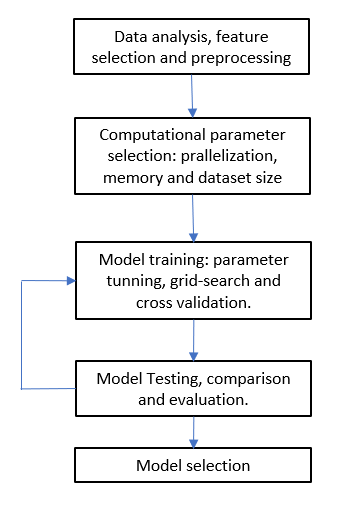
\includegraphics[width=0.5\linewidth]{TeX_files/Imagenes/general_met}
	\caption{General methodology for the project.}
	\label{fig:generalmet}
\end{figure}

\section{Data analysis and pre-processing}

The dataset consists of two files, one with the redshift measurement of DESI (TAR file) and the other with simulated true redshifts (TRUTH file). Apart from this, the files also contain several variables related to the parameters of the simulations, the class of a target, the observation conditions, etc. Since all of these variables represented as columns in the data files may not be important, we have to visualize and select which are important. 
\begin{figure}[h!]
	\centering
	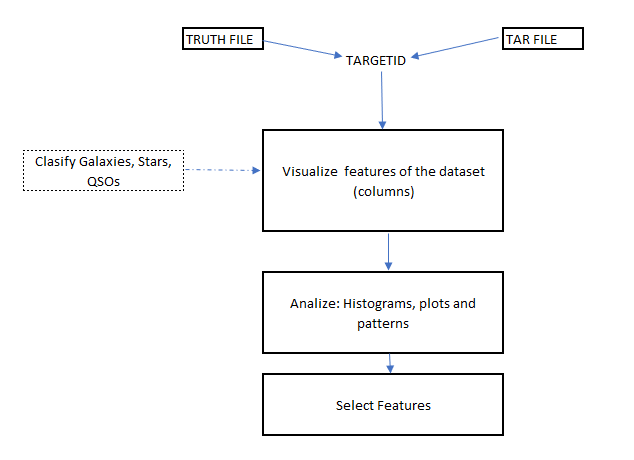
\includegraphics[width=0.8\linewidth]{TeX_files/Imagenes/metho_1}
	\caption{General methodology to understand the dataset and extract valuable features.}
	\label{fig:metho1}
\end{figure}

Figure \ref{fig:metho1} shows the step-by-step method to understand the data. In the first step, the two files have to be linked by the variable TARGETID, this variable represents the identity of a target through the whole pipeline of the experiments (observation and measurements). 

Next, we discriminate by target class (Galaxy, QSOs, etc...) and observe the behavior of the variables in the files with respect to redshift, for example, fluxes, magnitudes, etc ... From this, one can neglect some basic variables that contribute no relevant information to the problem. Then we execute a second analysis with more detail to see if the variables hold any relation with the redshift measurement by using histograms and approximating distributions. This is done to select which variables (or features) can be used to explain the differences between the true redshift of a galaxy and the redshift measured by DESI. The details of this can be found in Chapter \ref{Ch:Data}. 

After the features are selected,  we found that treating the variables in logarithmic scale is visually more representative and also produced good results in the machine learning algorithms. Since the kernel methods used are non-invariant to scaling, we also scale the data so that the means are equal to zero and the variance to one of all the variables.
\section{ High-performance computing analysis}
The training time of the model depends on the size of the training set, however, since the algorithms are going to be executed in parallel in the computing cluster of the University, the training time will also depend on the hardware. For example, the memory of the machine and the number of processors in which the code will be parallelized, as well as the number of processors that the computer (or node) actually has. To see what is the best combination of parameters to train the models in a reasonable amount of time up to a reasonable accuracy, it will be necessary to restrict also the size of the dataset used for training.

Figure \ref{fig:metho2} shows the step to accomplish this. First, we select the model and architecture (grid search/cross-validation, explained next) and the dataset size, in order to see how the training time scales with size, we  select different sizes, in this case, 100, 1000, 5000, and 10000 points. Then, the algorithm has to be run in a certain number of processors, and with certain RAM requested to the cluster, in this case, we try 1, 4, 8 and 16 processors, and 16, 32, 64 and 128 GB of memory. The expected result is the set of parameters to run the complete training algorithm on a big dataset. 
\begin{figure}[h!]
	\centering
	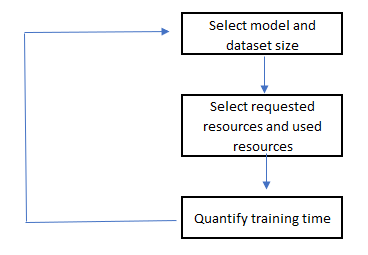
\includegraphics[width=0.7\linewidth]{TeX_files/Imagenes/metho_2}
	\caption{Sequence of steps to gather enough information to understend the relation between computation time, memory, dataset size and processors.}
	\label{fig:metho2}
\end{figure}

\section{Machine Learning}
Once we understand the scalability of the training time with respect to hardware variables, it is time to train and test the models. For this the dataset will be divided in a training set, corresponding to 75\% of the dataset and a test set (the rest 25 \%) as shown in Figure \ref{fig:metho3}. After this, according to the results of the previous section, we will split the training set into subsets of a specific size, these subsets will again be divided into a development and evaluation sets, to apply to them the grid search and cross-validation. We use cross-validation and grid search to select the hyper-parameters of the models and to quantify the error of the algorithms. 
\begin{figure}[h!]
	\centering
	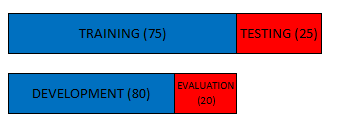
\includegraphics[width=0.6\linewidth]{TeX_files/Imagenes/metho_3}
	\caption{Divition of the dataset in train and test. The train set is divided in development-evaluation subsets.}
	\label{fig:metho3}
\end{figure}
\subsection{Training}
For training, we use grid search and cross validation to select the hyper-parameters of the models. Grid search executes an exhaustive search over specified parameters values for an estimator. The parameters are specified on a grid as follow:
\begin{verbatim}
param_grid = [
{'C': [1, 10, 100, 1000], 'kernel': ['linear']},
{'C': [1, 10, 100, 1000], 'gamma': [0.001, 0.0001], 'kernel': ['rbf']},
]
\end{verbatim}
this specifies that two grids should be explored: one with a linear kernel and C values in [1, 10, 100, 1000], and the second one with an RBF kernel, and the cross-product of C values ranging in [1, 10, 100, 1000] and gamma values in [0.001, 0.0001].

Learning the parameters of a prediction function and testing it on the same data is a methodological mistake: a model that would just repeat the labels of the samples that it has just seen would have a perfect score but would fail to predict anything useful on yet-unseen data. To avoid this, the grid search method is used alongside with \textbf{cross validation} (CV). In the \textit{k-fold} CV approach, the training set is divided into k smaller sets and the following procedure is followed for each of the k 'folds':
\begin{itemize}
	\item A model is trained using $k -1$ of the folds as training data (development, see Figure \ref{fig:metho3}).
	\item the resulting model is validated on the remaining part of the data (validation, see Figure \ref{fig:metho3})
\end{itemize}
The performance measure reported by k-fold cross-validation is then the average of the values computed in the loop. This approach can be computationally expensive.

\subsection{Testing}
Once we have trained the models, they will be tested on the unseen 25\% of the data to check its generalization ability. This means that we need to see whether the model truly 'learns' to predict redshifts or just memorized the training dataset. To select the best performing algorithm on the test dataset, the criterion will be the $r^2$ measure and the simplicity of the model.
\subsection{Model Performance}
The performance metric used to evaluate a model is the coefficient of determination, $r^2$ score. It provides a measure of how well future samples are likely to be predicted by the model, or the proportion of the variance in the dependent variable that is predictable from the independent variables. The best possible score is 1.0 and it can be negative (because the model can be arbitrarily worse). A constant model that always predicts the expected value of y, disregarding the input features, would get an $r^2$ score of 0.0 \cite{krr}.

If $\hat{y_i}$ is the predicted value of the \textit{i}-th sample and $y_i$ is the corresponding true value, then the score $r^2$ estimated over $n_{samples}$ is defined as 
\begin{equation}
r^2 (y, \hat{y}) = 1 - \frac{\sum_{i = 0}^{n_{samples} - 1} \left(y_i - \hat{y_i}\right)^2}{\sum_{i = 0}^{n_{samples} - 1} \left(y_i - \bar{y_i}\right)^2},
\end{equation} 
where $\bar{y} = \frac{1}{n_{samples}}\sum_{i = 0}^{n_{samples} - 1} y_i$. 

In general, the methodology for this project consists of analyzing the complete dataset and selecting the valuable features that can be used to predict (or recover) a correct redshift, finding the scalability of the training time with respect to the size of the dataset and the cluster resources, and finally, training an evaluating the machine learning models. 